\chapter{\label{chap:chap3} Proposta de trabalho}

Seguindo a organização arquitetural da Figura \ref{fig:fig1}, a proposta deste trabalho é fazer com que um \textit{fog node} conheça, de forma autônoma, os recursos disponibilizados por seus vizinhos.
Assim, cada \textit{fog node} saberá quais são os \textit{edge devices} disponíveis na rede, portanto,
o nodo que possui o sensor de chuva saberia que existe um outro nodo na rede capaz de medir a temperatura, por exemplo.


Podemos observar na topologia da Figura \ref{fig:fig1}, que os nodos não possuem um ponto centralizado de contato.
Em razão da topologia distribuída, se for necessário escalarmos a quantidade de nodos na rede, a mesma não deverá sofrer impactos significativos de performance.

Nas seções a seguir abordaremos a arquitetura, módulos e submódulos que compõem o projeto, bem como resultados esperados, validações e cenários de teste. 

\begin{figure}[htb!]
    \centering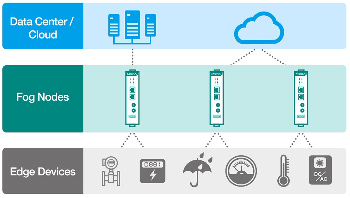
\includegraphics[width=.75\textwidth]{fig1.pdf}
    \caption
    {\label{fig:fig1} Organização arquitetural.} \cite{archfog:2017}
\end{figure}

\section{Arquitetura}

Esta seção define a pilha de protocolos a serem utilizados neste projeto, bem como a justifica pela escolha dos mesmos.
A pilha de protocolos atuará em conjunto com a organização arquitetural previamente definida na Figura \ref{fig:fig1}.

A fim de facilitar a compreensão da arquitetura deste projeto, a Figura \ref{fig:fig2} explicita a pilha de protocolos que o projeto fará uso para implementar as funcionalidades propostas.

\begin{figure}[htb!]
    \centering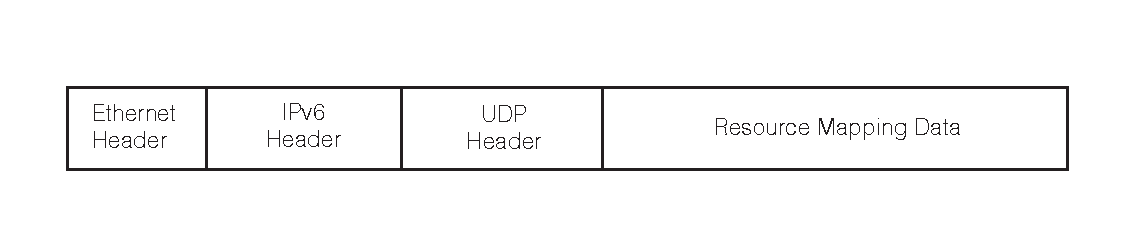
\includegraphics[width=.75\textwidth]{fig2.pdf}
    \caption%[This figure has a shorter caption now]%
    {\label{fig:fig2} Pilha de protocolos.}
\end{figure}

Dispondo do modelo de referência TCP/IP, constituido de cinco camadas: física, enlace, rede, transporte e aplicação \cite{tanenbaum2011redes}.
Este projeto utilizará IPv6 no nível de rede e UDP no nível de transporte.

[REVER] A utilização de IPv6 na camada de rede justifica-se pela grande quantidade de endereços válidos na internet que o protocolo provê, pois após o firmamento da internet das coisas é possível que cada dispositivo tenha um endereço IP único.
Sendo assim, a escalabilidade, no que diz respeito a quantidade de endereços, está garantida.[REVER]

Manter todos os nodos conectados, utilizando TCP por exemplo, despenderia uma quantidade de trafego significativo na rede. Além disso, o intuito desta implementação é transitar uma pequena quantidade de dados a cada requisição.
Portanto a utilização de datagramas UDP faz sentido neste projeto.

O protocolo proposto, entitulado \textit{Resource Mapping} na Figura \ref{fig:fig2}, atuará na camada de aplicação do modelo de referência TCP/IP \cite{tanenbaum2011redes} e será responsável por padronizar, descobrir e sincronizar os nodos da névoa.
Os maiores desafios neste modelo proposto são manter o estado global dos recursos acessível a todos os nodos, e garantir que o desempenho seja satisfatório com o objetivo permitir a escalabilidade da solução.



\section{Módulos}

De forma geral, cada nodo da rede deverá manter uma lista com os endereços IP`s que fazem parte do mapeamento.
Atrelado à cada endereço IP, deverá haver uma lista com os recursos providos por este.
Em vista disso, cada nodo portará um mapeamento global de recursos disponíveis na névoa.

O detalhamento das funcionalides que o projeto deverá dispor, bem como ilustrações relacionadas aos fluxos, serão abordadas nas proximas subseções.



\subsection{Middleware}

Observando a Figura \ref{fig:fig1}, notamos que há comunicação entre um fog node e seus respectivos edge devices.
A comunicação entre o fog node e seus edge devices não é o foco deste projeto e, portanto, será tratada de forma simulada.
Assim sendo, a simulação deverá prever alguns casos que, por vezes, possam suceder. Dentre alguns dos eventos possíveis está 
o acréscimo ou remoção de um edge device vinculado à algum fog node.

A manutenção dos recursos, acréscimo ou remoção, transcorrerá utilizando o protocolo CoAP.
Utilizar CoAP para estas funcionalidades faz sentido, uma vez que este prevê meios para vinculação de recursos à nodos.

Segundo a definição de POST protocolo CoAP temos que "a função real executada pelo método POST é determinada pelo servidor de origem e depende do recurso de destino.
Geralmente, resulta em um novo recurso sendo criado ou recurso de destino sendo atualizado"\cite{rfc7252}.
Já a mesma RFC define o método DELETE como "o método DELETE solicita que o recurso identificado pelo solicitação URI ser excluída"\cite{rfc7252}.

Nessa perspectiva, portanto, o uso do método POST faz sentido para gerarmos \textit{(CoRE) Link Format} e o método DELETE para removermos.


\subsection{Descoberta de recursos}


Partindo do pressuposto que os nodos da névoa já possuem seus recursos devidamente criados e acessíveis via CoAP,
como primeiro passo do mapeamento devemos considerar a entrada de um novo nodo, com seus recursos, na rede.
No momento em que o nodo dispor de um endereço IP válido, este deverá enviar um pacote para o endereço de broadcast indicando que possui recursos a serem disponibilizados.

%(tem como ou no broadcast deveria mandar ip junto?). interessados
Ao receberem o pacote enviado por broadcast, os nodos que desejarem saber quais recursos estão sendo providos por este novo membro, deverão realizar uma query
unicast para o endereço de origem indicando tal intenção.

Sendo assim, o nodo interessado deverá realizar uma query ao novo membro da rede, e esta query utilizará a URI \textit{/.well-known/core} do protocolo CoAP.
Lembrando que este fluxo de requisição e resposta, utilizando a URI \textit{/.well-known/core}, faz com que o nodo requisitado retorne todos seus recursos ao solicitante.

Para elucidarmos esta primeira fase do protocolo utilizaremos as imagens das Figuras \ref{fig:fig5} e \ref{fig:fig6} como exemplo de fluxo para a descoberta de recursos.

A topologia da névoa utilizada nas imagens é definida por fog nodes enumerados de um à cinco, sendo o nodo FN5 o ultimo a entrar na rede.
A figura \ref{fig:fig5} demonstra o nodo FN5 entrando na névoa e, portanto, deverá anunciar-se por broadcast indicando que possui recursos a serem disponibilizados.

\begin{figure}[htb!]
    \centering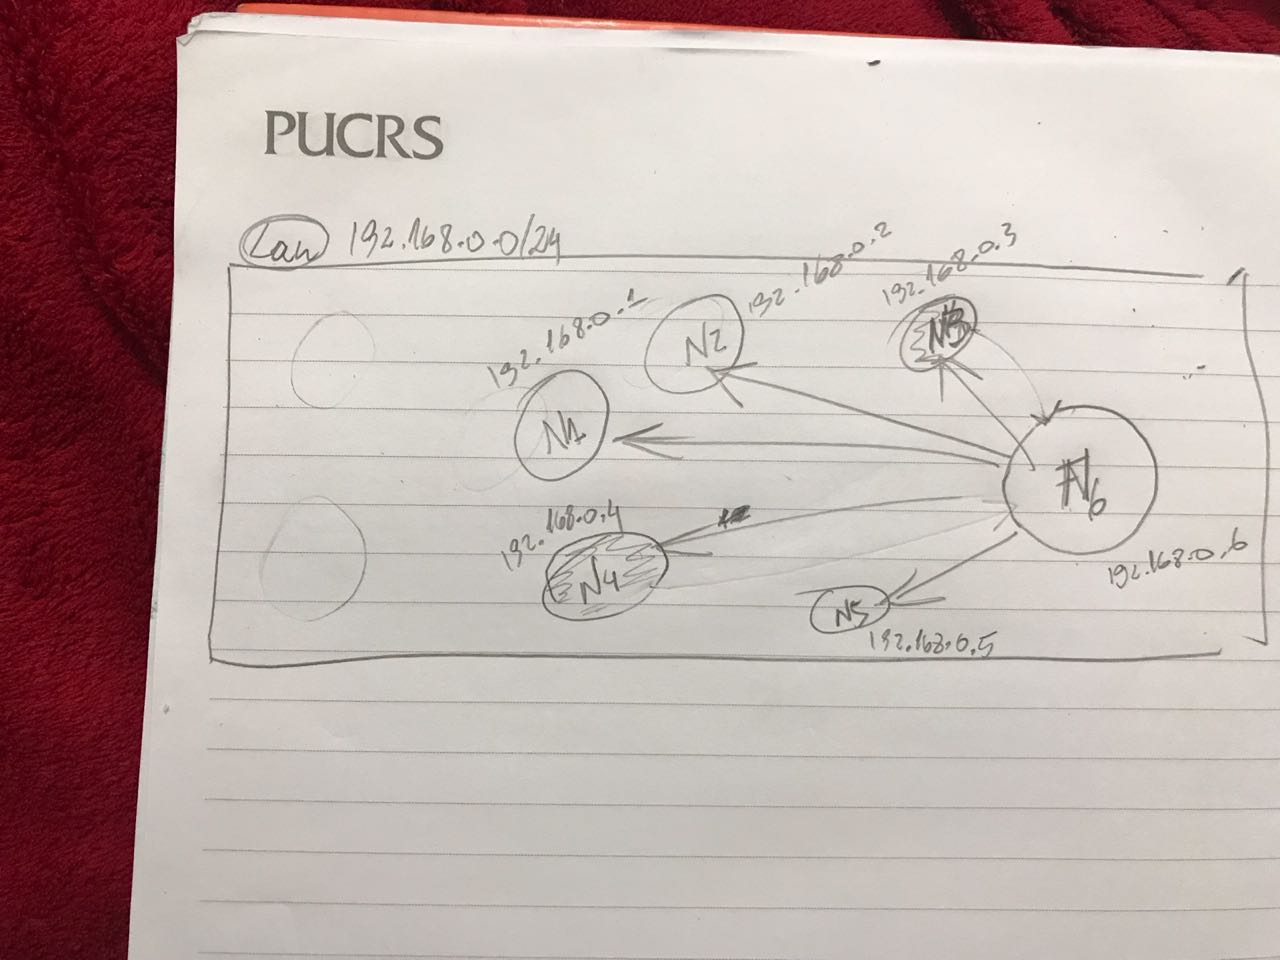
\includegraphics[width=.75\textwidth]{fig5.jpeg}
    \caption%[This figure has a shorter caption now]%
    {\label{fig:fig5} Nodo entrando na névoa.}
\end{figure}

Após FN5 enviar mensagem  "Hello" por broadcast, os nodos FN1, FN2 e FN3 realizam a query diretamente ao FN5 afim de obter os recuros disponíbilizados por ele.
Por não estar executada o protocolo de mapeamento, ou por não estar interessado em obter novos recursos, o nodo FN4 não realiza a query de descobrimento em FN5.


\begin{figure}[htb!]
    \centering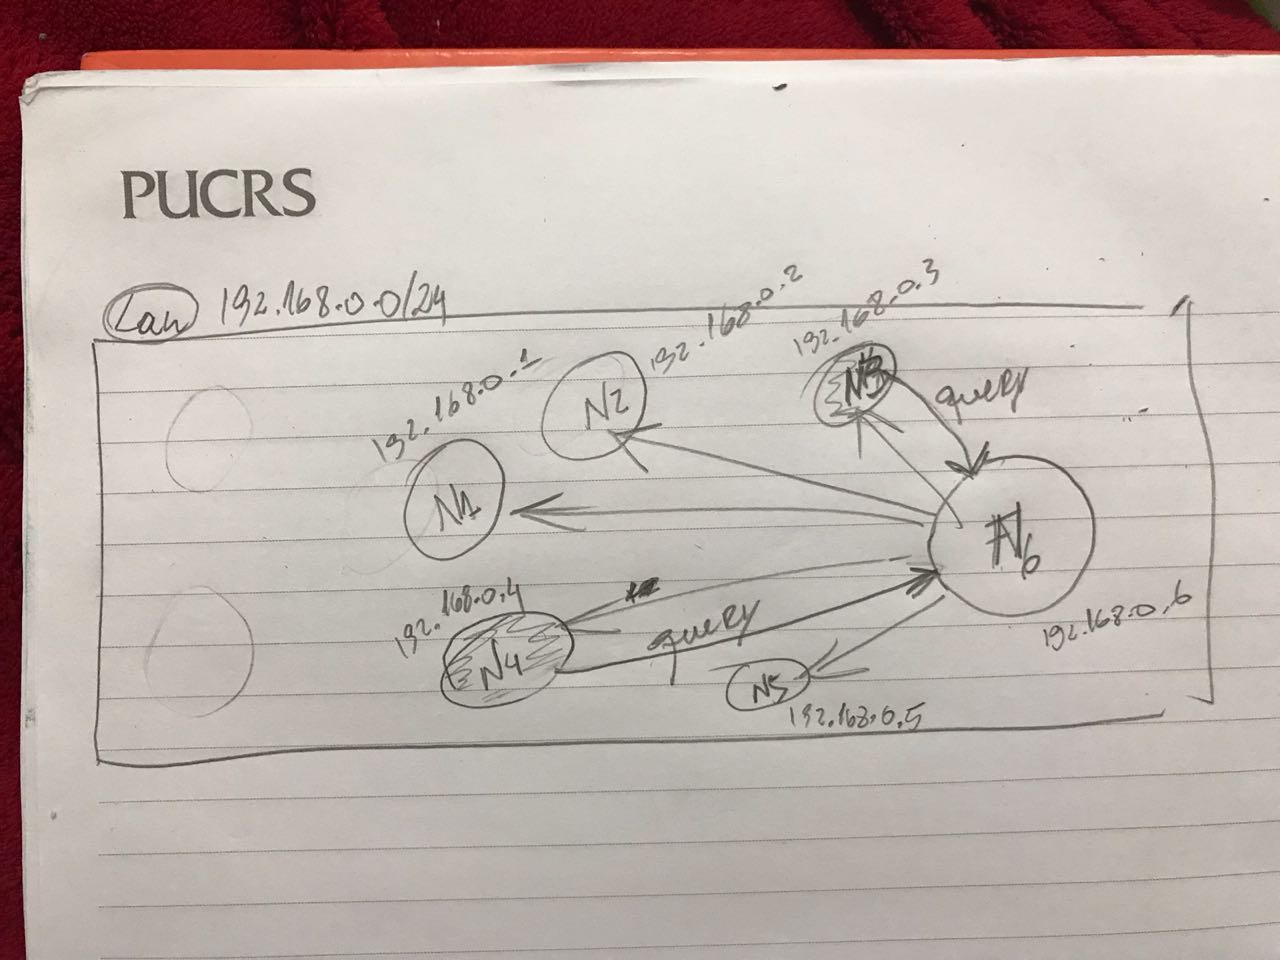
\includegraphics[width=.75\textwidth]{fig6.jpeg}
    \caption%[This figure has a shorter caption now]%
    {\label{fig:fig6} Nodos realizando query.}
\end{figure}

% ATENCAO
% nodo pode querer divulagar e nao usar..servidor,
% nodo pode querer só usar e nao divulgar.


\subsection{Gerenciamento de recursos}

A manutenibilidade da lista de recursos globais é relevante para que a implementação do protocolo tenha sucesso, pois a névoa deverá saber quando um nodo, ou recurso dele, deixou de fazer parte da rede.
Para tal, faz-se necessário a utilização de alguns mecanismos de controle.
Esses controles são realizados em duas esferas, uma trata do desvinculamento do nodo da rede e outra quando um recurso deixa de fazer parte dela.

O desvinculamento pode ser abordado de forma similar as mensagens de \textit{keep alive} utilizadas no protocolo BGP, por exemplo.
Mensagens de keep alive são adotadas para que os nodos da rede avisem seus vizinhos que ainda estão em operação, pois sem esse procedimento seria difícil
saber quando remover um IP da lista de recursos globais. Portanto, para manter a lista o mais atualizada possível, este protocolo implementará mensagens deste tipo.


%o que acontece quando nodo recebe resposta?




% \subsection{Politica de cache}
% Afim de eviar lalalal, este protocolo executara a politica de cache write back...


% Cada nodo da rede deve manter uma lista com os endereços IP`s que fazem parte do mapeamento. Juntamente à cada endereço IP, deverá haver uma lista com os recursos providos por ele.
% Em vista disso, cada nodo da névoa possui um mapeamento global de recursos disponíveis na rede.

% Quando um nodo entrar na rede pela primeira vez, deverá enviar um pacote para os endereços \textit{unicasts} indicando os recursos que disponibilizará.
% O Pseudocódigo \ref{alg:alg1} demonstra, de forma simplificada, a política de atualização que cada nodo deverá implementar.


% \begin{algorithm}[htb]
%     \begin{center}
%         \begin{algorithmic}[1]
%             \STATE \textbf{function} $\text{Police(ip, resources)}$
%             \STATE \hspace{\algorithmicindent} \textbf{if} $\text{exists(ip)}$
%             \STATE \hspace{\algorithmicindent} \hspace{\algorithmicindent} $\text{update(ip, resources)}$
%             \STATE \hspace{\algorithmicindent} \textbf{else}
%             \STATE \hspace{\algorithmicindent} \hspace{\algorithmicindent} $\text{insert(ip, resources)}$
%         \end{algorithmic}
%     \end{center}
%     \caption[Política de atualização de recursos]%
%         {\label{alg:alg1} Política de atualização de recursos.}%
%     \end{algorithm}


% No momento em que um nodo requisitar um recurso global da névoa, e este estiver fora de operação, o nodo que foi solicitado deverá enviar um novo pacote para os endereços \textit{unicasts} indicando quais são os seus recursos existentes no momento.
% O nodo solicitado percebe que este recurso não esta mais disponível porque recebeu na requisição o id do recurso, e este não está em sua lista local.
% Lembrando que o nodo requisitado está consciente desta divergência em virtude da execução continua dos métodos providos pelo \textit{middleware}. Portanto, o gatilho para a atualização dos recursos na névoa
% é disparado pelo primeiro nodo que requisitar um recurso inválido.


\section{Resultados esperados}

Espera-se que este trabalho resulte em um protocolo funcional a nível de prova de conceito e que seja capaz de descobrir, sincronizar e consumir recursos de dispositivos sob computação em névoa.
Além disso, temos como objetivo fazer com que a névoa configure-se de forma autônoma, ou seja, quando um recurso ou nodo entrar ou sair da rede, a mesma deverá manter-se coerente.


\section{Validação}

Para validarmos o funcionamento do protocolo, utilizaremos um simulador de dispositivos a ser definido no decorrer deste TCC.
Estes dispositivos executarão o \textit{middleware} citado no item 3.2.1 deste trabalho.

\section{Cenários de teste}

\begin{itemize}
    \item Entrada de algum equipamento na rede e este anunciando seus recursos. 
    \item Atualização das listas globais quando algum equipamento deixar de responder as mensagens de \textit{keep alive}.
    \item Utilização de recursos de nodos da rede.
    \item Desligamento de recursos de algum dispositivo da rede, e posterior a isso, a tentativa de acesso a esse recurso por algum nodo.
    O equipamento que perdeu o recurso deverá anunciar seus novos recursos atualizando a lista global dos outros nodos da névoa.
\end{itemize}










